% Options for packages loaded elsewhere
\PassOptionsToPackage{unicode}{hyperref}
\PassOptionsToPackage{hyphens}{url}
\documentclass[
  10pt,
  a4paper,
]{article}
\usepackage{xcolor}
\usepackage[margin=22mm]{geometry}
\usepackage{amsmath,amssymb}
\setcounter{secnumdepth}{-\maxdimen} % remove section numbering
\usepackage{iftex}
\ifPDFTeX
  \usepackage[T1]{fontenc}
  \usepackage[utf8]{inputenc}
  \usepackage{textcomp} % provide euro and other symbols
\else % if luatex or xetex
  \usepackage{unicode-math} % this also loads fontspec
  \defaultfontfeatures{Scale=MatchLowercase}
  \defaultfontfeatures[\rmfamily]{Ligatures=TeX,Scale=1}
\fi
\usepackage{lmodern}
\ifPDFTeX\else
  % xetex/luatex font selection
\fi
% Use upquote if available, for straight quotes in verbatim environments
\IfFileExists{upquote.sty}{\usepackage{upquote}}{}
\IfFileExists{microtype.sty}{% use microtype if available
  \usepackage[]{microtype}
  \UseMicrotypeSet[protrusion]{basicmath} % disable protrusion for tt fonts
}{}
\makeatletter
\@ifundefined{KOMAClassName}{% if non-KOMA class
  \IfFileExists{parskip.sty}{%
    \usepackage{parskip}
  }{% else
    \setlength{\parindent}{0pt}
    \setlength{\parskip}{6pt plus 2pt minus 1pt}}
}{% if KOMA class
  \KOMAoptions{parskip=half}}
\makeatother
\usepackage{graphicx}
\makeatletter
\newsavebox\pandoc@box
\newcommand*\pandocbounded[1]{% scales image to fit in text height/width
  \sbox\pandoc@box{#1}%
  \Gscale@div\@tempa{\textheight}{\dimexpr\ht\pandoc@box+\dp\pandoc@box\relax}%
  \Gscale@div\@tempb{\linewidth}{\wd\pandoc@box}%
  \ifdim\@tempb\p@<\@tempa\p@\let\@tempa\@tempb\fi% select the smaller of both
  \ifdim\@tempa\p@<\p@\scalebox{\@tempa}{\usebox\pandoc@box}%
  \else\usebox{\pandoc@box}%
  \fi%
}
% Set default figure placement to htbp
\def\fps@figure{htbp}
\makeatother
\setlength{\emergencystretch}{3em} % prevent overfull lines
\providecommand{\tightlist}{%
  \setlength{\itemsep}{0pt}\setlength{\parskip}{0pt}}
\usepackage{mathrsfs}
\usepackage{mathtools}
\usepackage{xurl}
\emergencystretch=3em
\setcounter{tocdepth}{1}
\newcommand{\Beta}{\mathrm{B}}
\DeclareUnicodeCharacter{00B2}{\ensuremath{^2}}
\DeclareUnicodeCharacter{00B1}{\ensuremath{\pm}}
\DeclareUnicodeCharacter{00D7}{\ensuremath{\times}}
\DeclareUnicodeCharacter{2192}{\ensuremath{\to}}
\DeclareUnicodeCharacter{21A6}{\ensuremath{\mapsto}}
\DeclareUnicodeCharacter{2208}{\ensuremath{\in}}
\DeclareUnicodeCharacter{2209}{\ensuremath{\notin}}
\DeclareUnicodeCharacter{2212}{\ensuremath{-}}
\DeclareUnicodeCharacter{2227}{\ensuremath{\wedge}}
\DeclareUnicodeCharacter{2228}{\ensuremath{\vee}}
\DeclareUnicodeCharacter{2260}{\ensuremath{\ne}}
\DeclareUnicodeCharacter{2264}{\ensuremath{\le}}
\DeclareUnicodeCharacter{2265}{\ensuremath{\ge}}
\DeclareUnicodeCharacter{2297}{\ensuremath{\otimes}}
\usepackage{bookmark}
\IfFileExists{xurl.sty}{\usepackage{xurl}}{} % add URL line breaks if available
\urlstyle{same}
\hypersetup{
  hidelinks,
  pdfcreator={LaTeX via pandoc}}

\author{}
\date{}

\begin{document}

{
\setcounter{tocdepth}{3}
\tableofcontents
}
\section{Actual signed-cover averaging and the supported-zero
endpoint}\label{actual-signed-cover-averaging-and-the-supported-zero-endpoint}

This calculation uses the original eight-state completion and its actual
monodromy. It proves that averaging either of the two retained trace
forms over that group produces a positive semidefinite form, calculates
the complete defect, and evaluates the change on actual Weil tests. The
group action belongs to the auxiliary quartic cover. Its action on an
arithmetic global trace is not asserted.

The original cover and its full monodromy are proved in
\href{https://github.com/KokunoYumeto/zeta-function-research-reader/blob/ab45e221579a0d48ce2885b4ecdf1a6aefc24a20/workbenches/splitzero-tandem/continuations/20260920-fable-boundary-action/FABLE_TO_ORIGINAL_CONDUCTOR.tex\#L2097}{\emph{The
ES--Fable inverse correspondence in the original weighted conductor},
SM1--SM19, source lines2097--2513}. The exact fibre, trace and
involutions used here are proved in
\href{https://github.com/KokunoYumeto/zeta-function-research-reader/blob/d5c9d198a8432e3ede468b280162a99c00e3f4f7/workbenches/splitzero-tandem/branches/tau-zero-prime-positivity/EIGHT_STATE_HEAT_COMPARISON.md}{\emph{The
original eight-state heat comparison}, ESH9--ESH34}. The actual test
convention is
\href{https://github.com/KokunoYumeto/zeta-function-research-reader/blob/d5c9d198a8432e3ede468b280162a99c00e3f4f7/workbenches/splitzero-tandem/branches/tau-zero-prime-positivity/WEIL_ES_COMPENSATION_DERIVATION.md}{\emph{The
actual Weil correction has the ES three-plus-one form}, WEC1--WEC5}. The
Gaussian theta map below proves the endpoint comparison directly,
retaining supported zero.

\subsection{1. Exact fibre and point
coordinates}\label{exact-fibre-and-point-coordinates}

At the unchanged target \(\mathbf U_*=(0,0,-1,0)\), the completed
algebra is \[
\mathcal A=\mathbb C[R,T]/(R^3-R,T^2-3R^2+1)
\ \times\ \mathbb C[\Theta]/(\Theta^2+1).
\tag{HWA1}
\] Its eight geometric points, in the order retained throughout, are \[
X=(0+,0-,1+,1-,-1+,-1-,\infty+,\infty-)
\tag{HWA2}
\] with coordinates
\((0,\pm i),(1,\pm\sqrt2),(-1,\pm\sqrt2),(\infty,\pm i)\). Evaluation is
an algebra isomorphism \(\operatorname{ev}:\mathcal A\to\mathbb C^X\).
Indeed, the root indicators are
\(e_0=1-R^2,e_1=(R^2+R)/2,e_{-1}=(R^2-R)/2\). Inside a finite root
factor with chosen positive sign coordinate \(t_j\), its point
indicators are \(e_j(1\pm T/t_j)/2\). The infinity indicators are
\((1\mp i\Theta)/2\). These eight orthogonal idempotents sum to one,
evaluate as the eight coordinate vectors, and supply the inverse.
Multiplication is diagonal in this basis, so \[
\operatorname{Tr}_{\mathcal A}(x)=\sum_{p\in X}x_p.
\tag{HWA3}
\] No coordinate weighting is discarded: the coefficient basis and point
basis are related by the exact map \[
(c_j,d_j)\longmapsto(c_j+t_jd_j,c_j-t_jd_j),
\quad(t_0,t_1,t_{-1},t_\infty)=(i,\sqrt2,\sqrt2,i).
\tag{HWA4}
\]

Let \(\Sigma\) negate every sign coordinate and let \(\kappa\) conjugate
coefficients. The original native map is \(J(R,T)=(-R,-T)\),
\(J(v,\Theta)=(-v,\Theta)\), where \(v=1/R\) on the reciprocal chart.
Combining each with coefficient conjugation gives the following point
permutations: \[
q_\Sigma=(1+\ 1-)(-1+\ -1-),
\quad
q_J=(1+\ -1-)(1-\ -1+)(\infty+\ \infty-).
\tag{HWA5}
\] For example, conjugation at root0 swaps \(i,-i\), after which either
\(\Sigma\) or \(J\) swaps them back. At infinity \(J\) fixes \(\Theta\),
so conjugation still swaps the two points. Formula(HWA5) follows on all
eight points. If \(Q_q\) denotes the permutation matrix of the
involution \(q\), then \[
B_q(x,y)=\operatorname{Tr}(x^{\#_q}y)=x^*Q_qy.
\tag{HWA6}
\] Thus \(B_J\) has inertia \((5,3,0)\) and \(B_\Sigma\) has inertia
\((6,2,0)\): each swapped pair contributes eigenvalues \(1,-1\), and
each fixed point contributes1. The point metric here is the exact sum in
the regular trace, not the ES source metric.

\subsection{2. The actual order-192 group and its
average}\label{the-actual-order-192-group-and-its-average}

Label the four root pairs by \(j=0,1,-1,\infty\). The group proved in
SM1--SM19 is \[
G=\{(\sigma,\pi):\pi\in S_4,\ \sigma\in\{\pm1\}^4,
\ \prod_j\sigma_j=\operatorname{sgn}\pi\},
\quad(j,\epsilon)\mapsto(\pi(j),\sigma_j\epsilon).
\tag{HWA7}
\] There are exactly \(24\cdot8=192\) elements. For completeness, its
appearance in the actual quartic is determined by \(a_j^2H'(r_j)=1\) and
the invariant \(A^2\prod_{j<k}(r_k-r_j)\prod_ja_j\in\{1,-1\}\).
Exchanging adjacent roots along semicircles makes the moving derivatives
turn through \(\pi\), so their square roots yield four-cycles
\((j+\ (j+1)+\ j-\ (j+1)-)\). Their squares generate all even sign
patterns, and their root permutations generate \(S_4\); this proves
equality with(HWA7), as calculated with exact paths and coordinates in
SM7--SM12. The completed cover is unramified at the infinity pair
because its reciprocal equations have determinant
\(2\Theta k'(0)=2\Theta\ne0\). Paths from a nearby point with \(A\ne0\)
to \(\mathbf U_*\) transport its eight separate local charts.
Relabelling the roots and their chosen signs conjugates(HWA7) by a
signed permutation, which preserves the determinant-one subgroup. We
therefore use that same exact group on(HWA2).

Let \(P_g\) be its permutation matrix on point functions. Define the
explicitly scaled finite conjugation sum \[
\mathscr E(Q)=\frac1{192}\sum_{g\in G}P_g^*QP_g.
\tag{HWA8}
\] The factor \(1/192\) is part of the definition, so the unit vector
\(\mathbf1\), whose original trace square is8, still has square8. Let \[
P_{\rm ev}=\frac{I+P_\Sigma}{2},\qquad
P_{\rm c}=\frac{\mathbf1\mathbf1^*}{8}.
\tag{HWA9}
\] These are orthogonal projections for the point metric, respectively
onto sign-even functions and constant functions. Their kernels and ranks
follow directly: \(P_{\rm ev}\) replaces both values in each pair by
their arithmetic mean, so it has rank4; \(P_{\rm c}\) replaces every
value by the mean of all eight, so it has rank1.

The two exact averages are \[
\boxed{\mathscr E(Q_\Sigma)=P_{\rm ev},\qquad
\mathscr E(Q_J)=\frac13P_{\rm ev}+\frac23P_{\rm c}.}
\tag{HWA10}
\] Here is a direct proof without an assumed irreducibility theorem. The
even-sign kernel \(K\subset G\) has eight elements. On the sign-even
subspace it acts trivially. On the four-dimensional sign-odd subspace it
acts by the four distinct sign characters. For two distinct root indices
\(j,k\), the average of \(\sigma_j\sigma_k\) over \(K\) is zero: choose
a third root \(l\ne j,k\), and multiply each sign pattern by the one
flipping \(j,l\), which pairs opposite contributions. Hence averaging a
matrix on that subspace over \(K\) removes all off-diagonal entries.
Averaging then over the root permutations makes its diagonal constant,
equal to one quarter of its trace.

Both original matrices commute with \(\Sigma\), so there are no
even--odd blocks. For \(Q_\Sigma\), the even block is \(I_4\) and the
odd block is \(\operatorname{diag}(1,-1,-1,1)\), of trace0. Its odd
average therefore vanishes. For \(Q_J\), the odd block is \[
\begin{pmatrix}1&0&0&0\\0&0&-1&0\\0&-1&0&0\\0&0&0&-1\end{pmatrix},
\tag{HWA11}
\] also of trace0. Its even block is the transposition exchanging roots1
and−1. Averaging its conjugates over \(S_4\) averages the six
transpositions. The resulting matrix has diagonal \(3/6=1/2\) and every
off-diagonal entry \(1/6\), because a given index is fixed by three
transpositions and a specified distinct pair is exchanged by one. This
is \(I_4/3+\mathbf1_4\mathbf1_4^*/6\). Transport through the exact even
projection gives(HWA10).

For \(s_j(x)=x_{j+}+x_{j-}\), the complete quadratic formulas are \[
\begin{aligned}
\overline B_\Sigma(x,x)&=\frac12\sum_j|s_j(x)|^2,\\
\overline B_J(x,x)&=\frac16\sum_j|s_j(x)|^2
 +\frac1{12}\left|\sum_js_j(x)\right|^2.
\end{aligned}
\tag{HWA12}
\] Thus each has inertia \((4,0,4)\). For the native average its
eigenvalues on constants, the three-dimensional even sum-zero subspace,
and the four-dimensional odd subspace are respectively \(1,1/3,0\).
Their common radical is exactly \[
V_{\rm odd}=\{x:x_{j-}=-x_{j+}\ \text{for all four }j\}.
\tag{HWA13}
\] These formulas exhibit positivity from the actual finite group,
retaining every root and sign coordinate in the projection and its
kernel.

\subsection{3. Exact defect and multiplication retained by the odd
space}\label{exact-defect-and-multiplication-retained-by-the-odd-space}

Define, on the original eight-dimensional space, \[
D_q=Q_q-\mathscr E(Q_q).
\tag{HWA14}
\] For \(\Sigma\), the defect vanishes on even functions and is exactly
\(\operatorname{diag}(1,-1,-1,1)\) on odd functions. Its inertia is
\((2,2,4)\). For \(J\), the even block has eigenvalues
\(0,2/3,2/3,-4/3\), and the odd block is(HWA11), with eigenvalues
\(1,1,-1,-1\). To verify the even values, the root transposition fixes
the constant line and has eigenvalues \(1,1,-1\) on its sum-zero
complement; subtract its average \(1/3\) on that complement.
Consequently \[
\operatorname{inertia}(D_J)=(4,3,1).
\tag{HWA15}
\] The exact comparison for arbitrary vectors is \[
B_q(x,y)=\overline B_q(x,y)+x^*D_qy.
\tag{HWA16}
\] The average cannot be the regular trace paired with an antilinear
algebra involution on the original reduced \(\mathcal A\). Such an
involution permutes its eight primitive idempotents and conjugates their
coefficients; its trace matrix is an invertible permutation matrix
by(HWA3). The matrices in(HWA10) have rank4. This proves the stated
nonidentification and also identifies its exact four-dimensional
radical.

There is an explicit linear receiver and an exact multiplication defect.
Put \[
E:\mathbb C^X\to\mathbb C^4,
\quad E(x)_j=(x_{j+}+x_{j-})/2,
\quad O(x)_j=(x_{j+}-x_{j-})/2,
\tag{HWA17}
\] and let \(I:\mathbb C^4\to\mathbb C^X\) duplicate each root value.
Then \(EI=\operatorname{id}\), \(IE=P_{\rm ev}\),
\(\ker E=V_{\rm odd}\), and \[
E(xy)=E(x)E(y)+O(x)O(y).
\tag{HWA18}
\] All products on the right are coordinatewise. Expanding
\((a_j\pm b_j)(c_j\pm d_j)\) proves the identity in every coordinate.
Thus \(E\) is a retraction of vector spaces and a bimodule map over the
embedded sign-even algebra, while its displayed second term records
every product returning from odd to even support. In particular
\(z=e_{0+}-e_{0-}\) has \(E(z)=0\) but \(E(z^2)=e_0\ne0\). The kernel is
not an ideal, and(HWA17) is not silently promoted to an algebra
quotient.

The average forms factor exactly through \(E\): \[
\overline B_\Sigma(x,y)=2\sum_j\overline{E(x)_j}E(y)_j,
\quad
\overline B_J(x,y)=\frac23\sum_j\overline{E(x)_j}E(y)_j
 +\frac13\overline{\sum_jE(x)_j}\sum_jE(y)_j.
\tag{HWA19}
\] For any retained support lattice, applying these linear amplitude
maps to a supported module keeps its support coordinate unchanged. An
amplitude sent to0 therefore lands at the supported-zero element of that
same support, not at the unsupported element \(\tau\). Formula(HWA18)
remains the precise reason that this amplitude projection is not a
semiring homomorphism.

The average of vectors is a third, separately specified map: \[
\frac1{192}\sum_gP_gx=P_{\rm c}x,
\quad B_q(P_{\rm c}x,P_{\rm c}y)=x^*P_{\rm c}y.
\tag{HWA20}
\] The first identity follows because the group acts transitively on the
eight states, so each target coordinate receives each source coordinate
equally often. The second uses \(Q_q\mathbf1=\mathbf1\). This rank-one
form differs from both rank-four forms(HWA10); all three maps and their
different kernels are explicit.

\subsection{4. Actual supported-zero theta
endpoints}\label{actual-supported-zero-theta-endpoints}

Keep \(\mathcal T=C_c^\infty(\mathbb R;\mathbb C)\) and the programme
convention \[
M_f(s)=\int_{\mathbb R}f(v)e^{-(s-1/2)v}\,dv,
\qquad f^\#(v)=\overline{f(-v)}.
\tag{HWA21}
\] The transform of \(f^\#\) is \(\overline{M_f(1-\bar s)}\), by the
substitution \(v\mapsto-v\). Define the even Schwartz function \[
\phi_f(x)=\int_{\mathbb R}e^{v/2}f(v)e^{-\pi e^{2v}x^2}\,dv.
\tag{HWA22}
\] If \(\operatorname{supp}f\subset[-R,R]\), every derivative in \(x\)
of the integrand is a polynomial in \(x\) with bounded coefficients
times a Gaussian bounded by a constant times \(e^{-\pi e^{-2R}x^2}\).
Integration proves every Schwartz bound. The Fourier convention
\(\widehat\phi(y)=\int\phi(x)e^{-2\pi ixy}dx\) gives \[
\phi_f(0)=M_f(0),\quad \int\phi_f=M_f(1),
\quad\widehat{\phi_f}=\phi_{f(-\cdot)},
\quad\widehat{\overline{\phi_f}}=\phi_{f^\#}.
\tag{HWA23}
\] For the integral use \(\int e^{-\pi e^{2v}x^2}dx=e^{-v}\). For
Fourier use the same Gaussian scaling and substitute \(v\mapsto-v\).
Absolute integrability from the compact \(v\)-support justifies both
interchanges.

In \(G(\mathbb Z)=\{\tau\}\sqcup\mathbb Z\), let \(e\) denote
supported0. Its principal ideal \(\{\tau,e\}\) is prime: a product of
two nonzero supported integers is again nonzero supported, so a product
in that ideal has at least one factor there. The full supported theta is
\[
\Theta_f(x)=\sum_{n\in\mathbb Z}\phi_f(nx),\quad x>0,
\tag{HWA24}
\] and retains the \(n=0\) summand \(\phi_f(0)\) as the \(e\)-term. The
external \(\tau\) is a different label; no integer in this sum
represents it. Poisson summation for this Schwartz function gives
\(\Theta_f(x)=x^{-1}\Theta_{f(-\cdot)}(x^{-1})\). For this particular
mixture the identity follows directly by integrating the Gaussian theta
identity, with uniform absolute convergence for \(v\) in the compact
support. Its two endpoint amplitudes are exactly(HWA23), not an
arbitrary selected pair of complex numbers. Their regularized Mellin
endpoint terms are \[
-\frac{M_f(0)}s+\frac{M_f(1)}{s-1}.
\tag{HWA25}
\] Indeed split the integral of \(\Theta_f(x)-\phi_f(0)\) at1; use full
Poisson on \((0,1)\), and integrate \(x^{s-1}(x^{-1}M_f(1)-M_f(0))\).
Initially these elementary integrals converge for
\(\operatorname{Re}s>1\), and their displayed meromorphic expressions
supply continuation. The remaining transformed integrals over
\([1,\infty)\) are entire by rapid decay. Also direct Gaussian
integration in the initial half-plane gives \[
\int_0^\infty (\Theta_f(x)-\phi_f(0))x^{s-1}dx
=\pi^{-s/2}\Gamma(s/2)\zeta(s)M_f(s).
\tag{HWA26}
\] The two integer signs contribute2, cancelling the \(1/2\) in the
Gaussian Mellin integral. Uniform absolute convergence for
\(\operatorname{Re}s>1\) proves the exchange. This establishes both the
arithmetic amplitude and the exact endpoint residues from the retained
supported-zero theta.

For two actual tests the endpoint Hermitian pairing is \[
P_e(f,g)=\overline{M_f(0)}M_g(1)+\overline{M_f(1)}M_g(0).
\tag{HWA27}
\] This is the trace of the two-weight endpoint module with its Fourier
reflection exchanging the weights. It is the supported-zero endpoint
term; it is not all of the integrated Weil distribution. The separate
construction SZW retains the remaining finite-prime, archimedean and
fixed-support terms.

\subsection{5. Exact endpoint embedding and the change caused by
holonomy
averaging}\label{exact-endpoint-embedding-and-the-change-caused-by-holonomy-averaging}

Set \(A_f=M_f(0)\), \(B_f=M_f(1)\) and define \[
j:\mathcal T\to\mathbb C^X,
\quad j(f)=(0,0,A_f/\sqrt2,A_f/\sqrt2,
B_f/\sqrt2,B_f/\sqrt2,0,0).
\tag{HWA28}
\] The root assignment is stated in(HWA2): the two endpoint weights are
inserted into roots1 and−1. It is a linear comparison with scale
\(1/\sqrt2\), not a unital algebra map. By(HWA5),(HWA21), \[
j(f^\#)=\#_Jj(f),\qquad
B_J(j(f),j(g))=P_e(f,g).
\tag{HWA29}
\] Both formulas follow by exchanging \(A,B\) and conjugating; the two
signs at each root have equal values. Thus this is an exact
involution-preserving embedding of the two-dimensional endpoint quotient
into the actual completed trace.

The endpoint map \(f\mapsto(A_f,B_f)\) is onto. Here is a complete
section. Choose a positive smooth compact bump \(\psi\) on an open
interval. Put \(k_0(v)=e^{v/2}\), \(k_1(v)=e^{-v/2}\),
\(G_{ab}=\int\psi k_a\overline{k_b}\). For \(z\ne0\), the nonzero
combination \(\bar z_0e^{v/2}+\bar z_1e^{-v/2}\) cannot vanish on an
interval: multiplying by \(e^{v/2}\) would make \(\bar z_0e^v+\bar z_1\)
identically zero, whose derivative forces \(z_0=z_1=0\). Hence \(G\) is
positive definite. The function
\(S(A,B)=\psi\sum_b(G^{-1}(A,B)^T)_b\overline{k_b}\) has precisely those
two transforms by multiplication with \(G\). It is smooth and compactly
supported, proving surjectivity and \(\ker j=\{M_f(0)=M_f(1)=0\}\).

Substituting(HWA28) in(HWA12) gives the averaged endpoint form \[
\overline P_e(f,f)=\frac12(|A_f|^2+|B_f|^2)
 +\frac13\operatorname{Re}(\overline{A_f}B_f).
\tag{HWA30}
\] Its matrix is
\(\left(\begin{smallmatrix}1/2&1/6\\1/6&1/2\end{smallmatrix}\right)\),
with eigenvalues \(2/3,1/3\), so it is strictly positive on the endpoint
quotient. The exact change is \[
K_e=\overline P_e-P_e,
\quad
K_e(f,f)=\frac12(|A_f|^2+|B_f|^2)
-\frac53\operatorname{Re}(\overline{A_f}B_f).
\tag{HWA31}
\] In the explicitly related coordinates
\(u=(A+B)/\sqrt2,v=(A-B)/\sqrt2\), \[
P_e=|u|^2-|v|^2,
\quad\overline P_e=\frac23|u|^2+\frac13|v|^2,
\quad K_e=-\frac13|u|^2+\frac43|v|^2.
\tag{HWA32}
\] Thus actual tests with \((A,B)=(1,-1)\) have old value−2 and averaged
value \(2/3\), while tests with \((A,B)=(1,1)\) have old value2 and
averaged value \(4/3\). The section just proved supplies both tests. The
change has both signs on admissible tests, and its radical on
\(\mathcal T\) is exactly \(\ker j\): its two-dimensional matrix is
invertible and the section detects every nonzero endpoint vector.

The root-pair image of \(j\) is not invariant under the full group: a
signed root permutation taking root1 to root0 sends a vector with
\(A\ne0,B=0\) outside it. Such a permutation is in(HWA7) after choosing
signs with product equal to its permutation sign. This proves a specific
failure of invariance of this comparison map, with the group action and
endpoint map explicitly retained. It does not assert that every other
arithmetic comparison fails.

The full supported-zero construction
\href{https://github.com/KokunoYumeto/zeta-function-research-reader/blob/adfbfe74fa49e31cb7aa068cf755fb083be37c32/workbenches/splitzero-tandem/branches/tau-zero-prime-positivity/SUPPORTED_ZERO_PRIME_WEIL_DERIVATION.md}{\emph{The
supported-zero prime in the full theta and Weil trace distribution},
SZW24--SZW42} proves the actual integrated formula. Here are its
explicit terms and their exact transport. Put \(h=f^\#*g\), \(H=M_h\),
and retain \[
\begin{aligned}
\mathcal Z(f,g)&=\sum_\rho m_\rho\overline{M_f(1-\bar\rho)}M_g(\rho),\\
\mathcal A_\infty(f,g)&=\frac1{2\pi}\int_{\mathbb R}
\overline{\widehat f(t)}\widehat g(t)
\bigl(\operatorname{Re}\psi(1/4+it/2)-\log\pi\bigr)\,dt,\\
\mathcal P_{\rm fin}(f,g)&=\sum_{p,k\ge1}(\log p)p^{-k/2}
\{h(k\log p)+h(-k\log p)\}.
\end{aligned}
\tag{HWA33}
\] The sum in the last line is over primes \(p\) and integers \(k\ge1\).
It is finite for each compactly supported \(h\). The absolutely
convergent zero sum and archimedean integral, with their complete proof
and the original minus-exponent convention, are SZW24--SZW32.
Substituting \(P_e=\overline P_e-K_e\) gives the actual equality \[
\boxed{\mathcal Z=P_e+\mathcal A_\infty-\mathcal P_{\rm fin}
=\overline P_e+\mathcal A_\infty-\mathcal P_{\rm fin}-K_e.}
\tag{HWA34}
\] Formula(HWA31) gives the entire changed term on every admissible
test. In particular the negative endpoint \(-2\) becomes \(2/3\), while
its retained complement changes by \(-8/3\). This is an exact
calculation inside the derived supported-zero formula.

The full labels can be kept before any scalar projection. Let \(L\) be
the finite fixed-support lattice of SZW10--SZW13, \(\mathbf e_1\) its
top coordinate, and
\(\mathbf s_< =\sum_{\lambda\ne1}\mathbf e_\lambda\). Here lower labels
are distinct fixed zero points, not the independently different
coordinatewise adelic support construction. The original labelled
formula, now on \(h=f^\#*g\), is \[
\begin{aligned}
\boldsymbol B&=P_e\mathbf e_1+H(0)\mathbf s_<,\\
\boldsymbol D&=(\mathcal P_{\rm fin}-\mathcal A_\infty)\mathbf e_1+H(0)\mathbf s_<,\\
\boldsymbol B-\mathcal Z\mathbf e_1&=\boldsymbol D.
\end{aligned}
\tag{HWA35}
\] Keeping these lower fixed distributions exactly and applying the
holonomy comparison at the top endpoint gives \[
\begin{aligned}
\overline{\boldsymbol B}&=\overline P_e\mathbf e_1+H(0)\mathbf s_<,\\
\overline{\boldsymbol D}&=(\mathcal P_{\rm fin}-\mathcal A_\infty+K_e)\mathbf e_1
 +H(0)\mathbf s_<,\\
\overline{\boldsymbol B}-\mathcal Z\mathbf e_1&=\overline{\boldsymbol D}.
\end{aligned}
\tag{HWA36}
\] This follows by adding precisely \(K_e\mathbf e_1\) to both sides
of(HWA35). No lower support trace was merged with the top endpoint or
discarded.

For the minimal Fourier-closed endpoint module proved in SZW40--SZW42,
every lower fixed constant acquires its exact weight-one Dirac partner.
Its labelled boundary and geometric distributions are \[
\boldsymbol B^{\mathcal F}=P_e(\mathbf e_1+\mathbf s_<),\quad
\boldsymbol D^{\mathcal F}=(\mathcal P_{\rm fin}-\mathcal A_\infty)\mathbf e_1+P_e\mathbf s_<.
\tag{HWA37}
\] There is now the defined direct-sum comparison
\(\bigoplus_{\lambda\in L}j\) from the independent endpoint tests into
one completed eight-state vector space for each label. Averaging its
native forms label by label and restricting back to the diagonal actual
scalar tests gives \[
\begin{aligned}
\overline{\boldsymbol B}^{\mathcal F}&=\overline P_e(\mathbf e_1+\mathbf s_<),\\
\overline{\boldsymbol D}^{\mathcal F}&=
(\mathcal P_{\rm fin}-\mathcal A_\infty+K_e)\mathbf e_1
 +\overline P_e\mathbf s_<,\\
\overline{\boldsymbol B}^{\mathcal F}-\mathcal Z\mathbf e_1
&=\overline{\boldsymbol D}^{\mathcal F}.
\end{aligned}
\tag{HWA38}
\] Proof: add \(K_e\) on every label in(HWA37), using the original
identity
\(\boldsymbol B^{\mathcal F}-\mathcal Z\mathbf e_1=\boldsymbol D^{\mathcal F}\).
The direct-sum comparison is a specified linear map, and(HWA29) proves
its involution compatibility on each summand. The group is the actual
auxiliary-cover group on each receiver; no unproved action on the
arithmetic zeros or on the original test space has been introduced. Thus
the positive averaged boundary, its full geometric correction, the
supported-zero prime, the unsupported coordinate and every mixed-support
label are retained in one exact identity.

\begin{figure}
\centering
\pandocbounded{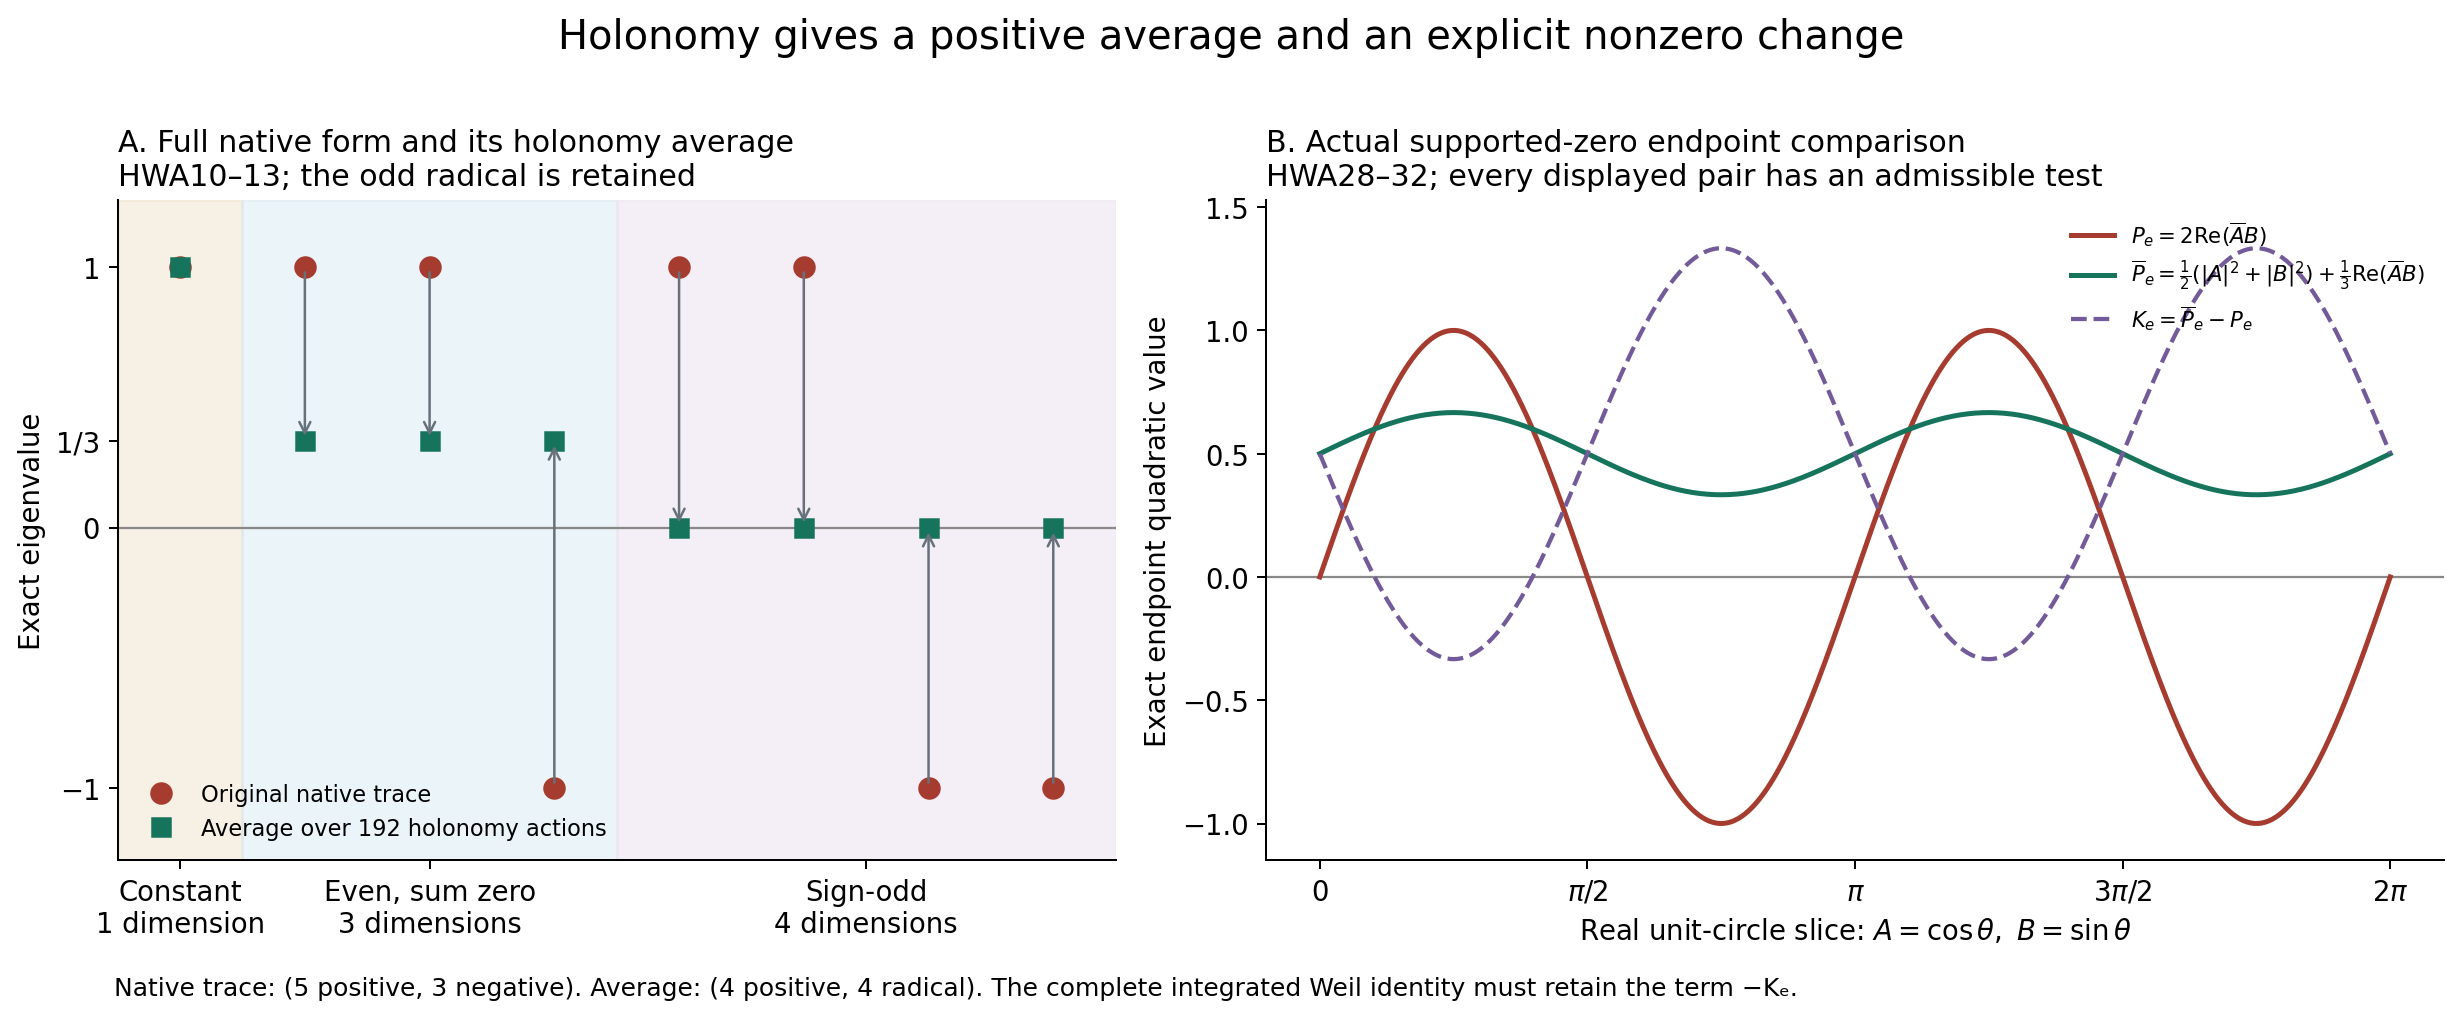
\includegraphics[keepaspectratio,alt={The complete native trace spectrum before and after its order-192 holonomy average, and the exact supported-zero endpoint comparison on actual admissible tests. HWA10--HWA15 prove the left panel; HWA28--HWA32 prove the right panel; HWA34--HWA38 retain its change in the full supported-zero formula.}]{figures/31_holonomy_endpoint_average.png}}
\caption{The complete native trace spectrum before and after its
order-192 holonomy average, and the exact supported-zero endpoint
comparison on actual admissible tests. HWA10--HWA15 prove the left
panel; HWA28--HWA32 prove the right panel; HWA34--HWA38 retain its
change in the full supported-zero formula.}
\end{figure}

\end{document}
